\section{System Design}

% Lead owner: Keerthi
% Section 5.7 owner: Sreeja

PBCP follows a Prevent -> Correct -> Learn pipeline. The system first infers what
the workload is trying to do, estimates whether the request is likely to waste
compute, and applies a pre-billing intervention when the expected savings justify
the action. Once a workload is running, PBCP continues to monitor for divergence
between declared intent and observed behavior, applies runtime corrections when
needed, and feeds those outcomes back into future governance decisions.

\subsection{Overview}

Open this subsection with the full pipeline narrative:
natural-language workload -> intent inference -> similarity retrieval ->
pre-execution simulation -> EV decision engine -> runtime optimizer ->
CPS/IFS tracking -> policy learning loop.
Figure~\ref{fig:architecture} presents this pipeline as the core
Prevent~$\rightarrow$~Correct~$\rightarrow$~Learn control loop.

\begin{figure}[t]
\centering
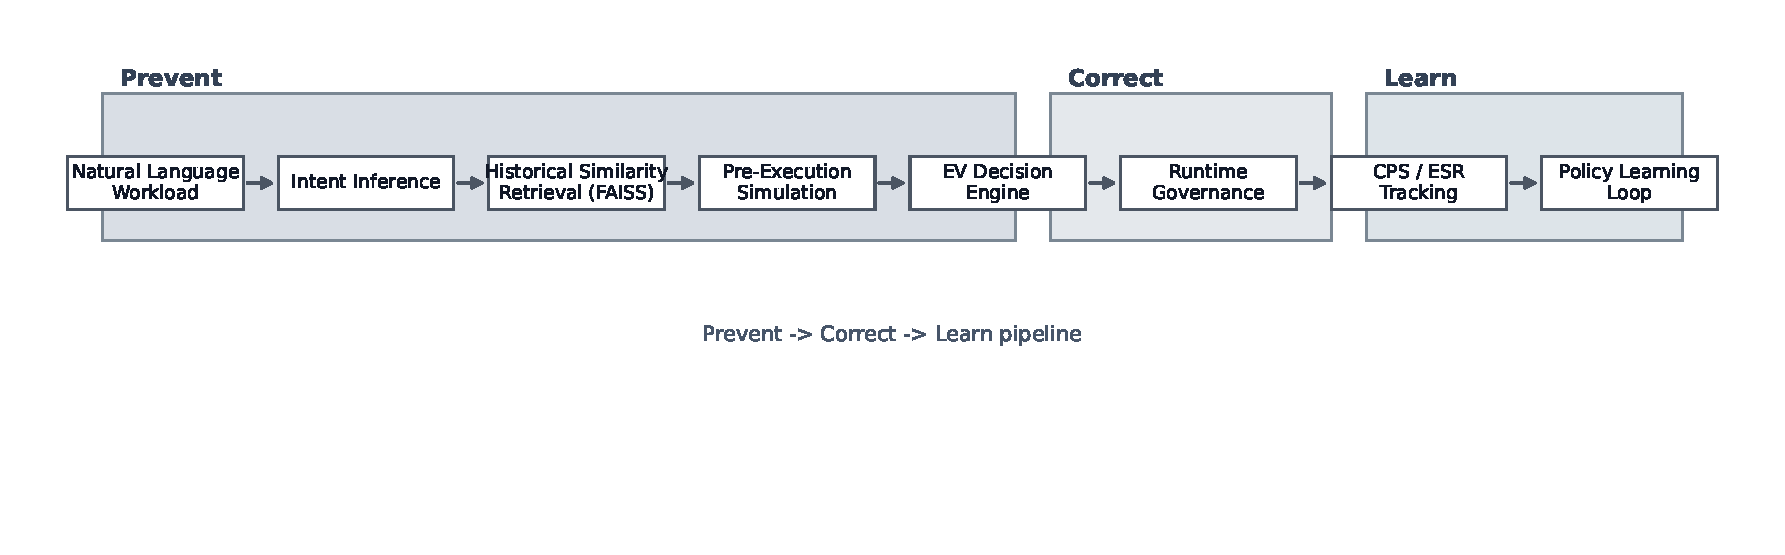
\includegraphics[width=\linewidth]{figures/architecture_overview.pdf}
\caption{PBCP system architecture. The pipeline groups pre-billing prevention, runtime correction, and policy learning into one governance loop.}
\label{fig:architecture}
\end{figure}

\subsection{Intent Inference}

Explain how workload descriptions, metadata, and team history are mapped into a
structured workload representation. Keep the emphasis on governance usefulness:
the purpose of intent inference is to surface the expected job type, recurrence,
sensitivity, urgency, and resource profile before execution begins.

\subsection{Historical Similarity Retrieval}

Describe FAISS-based nearest-neighbor retrieval over historical workload
representations. This subsection should explain how similar prior workloads
provide empirical priors for expected utilization, duration, and waste patterns,
including a cold-start fallback when close matches are unavailable.

\subsection{Pre-Execution Simulation}

Describe the simulator as the mechanism that projects likely utilization, cost,
and waste before provisioning. The narrative should stay systems-oriented: the
simulator turns intent plus historical priors into an estimate of what will
happen if the current request is allowed to execute unchanged.

\subsection{EV Decision Engine}

Explain the decision-theoretic intervention model. This subsection should compare
the expected value of BLOCK, AUTO\_CORRECT, SUGGEST, and PASS by balancing
prevented cost against intervention cost, delay risk, and failure risk.

\subsection{Runtime Governance}

Describe how PBCP responds after launch when hidden failures or prolonged idle
periods appear. This subsection should show runtime correction as a second line
of defense, not the primary contribution: runtime actions matter because some
divergence is only visible after execution starts.

\subsection{Intent-Behavior Discrepancy (IBD)}

This subsection is Sreeja's primary systems contribution. Define the
Intent-Behavior Discrepancy framing and the Intent-Fit Score as the semantic
alignment signal between inferred workload intent and observed runtime behavior.
Keep the canonical definition stable and use dashboard sub-scores only for
interpretability.

% Owner: Sreeja
% TODO(Sreeja): add final Section 5.7 prose defining intent-behavior divergence
% and IFS as the workload-alignment signal.


\subsection{Policy Learning Loop}

Close the design section with the learning loop. Explain how repeated divergence,
missed savings, and successful interventions update future governance policy so
the system improves over time rather than remaining a fixed rule set.
